\documentclass[10pt,letterpaper]{article}
\usepackage[top=0.85in,left=2.75in,footskip=0.75in]{geometry}

% Use adjustwidth environment to exceed column width (see example table in text)
\usepackage{changepage}

% Use Unicode characters when possible
\usepackage[utf8]{inputenc}

% textcomp package and marvosym package for additional characters
\usepackage{textcomp,marvosym}

% fixltx2e package for \textsubscript
\usepackage{fixltx2e}

% amsmath and amssymb packages, useful for mathematical formulas and symbols
\usepackage{amsmath,amssymb}

% cite package, to clean up citations in the main text. Do not remove.
%\usepackage{cite}

% Use nameref to cite supporting information files (see Supporting Information section for more info)
\usepackage{nameref,hyperref}

% line numbers
\usepackage[right]{lineno}

% ligatures disabled
\usepackage{microtype}
\DisableLigatures[f]{encoding = *, family = * }

% rotating package for sideways tables
\usepackage{rotating}

% Remove comment for double spacing
%\usepackage{setspace} 
%\doublespacing

% Text layout
\raggedright
\setlength{\parindent}{0.5cm}
\textwidth 5.25in 
\textheight 8.75in

% Bold the 'Figure #' in the caption and separate it from the title/caption with a period
% Captions will be left justified
\usepackage[aboveskip=1pt,labelfont={sf,bf},labelsep=space,justification=raggedright,singlelinecheck=off]{caption}

% Use the PLoS provided BiBTeX style
\usepackage[sort&compress,numbers]{natbib}
\renewcommand{\bibsection}{\begin{flushleft} \textsf{\Large{References}} \end{flushleft}}

% Remove brackets from numbering in List of References
%\makeatletter
%\renewcommand{\@biblabel}[1]{\quad#1.}
%\makeatother

% Leave date blank
\date{}

% Header and Footer with logo
\usepackage{lastpage,fancyhdr,graphicx}
\pagestyle{myheadings}
\pagestyle{fancy}
\fancyhf{}
\lhead{\sf Wagner et al (June 2018) -- \textbf{Mass Balance along Greenland Glacier Front}}
\rfoot{\thepage/\pageref{LastPage}}
\renewcommand{\footrule}{\hrule height 2pt \vspace{2mm}}
\fancyheadoffset[L]{2.25in}
\fancyfootoffset[L]{2.25in}
%\lfoot{\sf PLOS}

\renewcommand{\d}[2]{\frac{d #1}{d #2}} % for derivatives
\newcommand{\dd}[2]{\frac{d^2 #1}{d #2^2}} % for double derivatives
\newcommand{\pd}[2]{\frac{\partial #1}{\partial #2}} 
\newcommand{\pdd}[2]{\frac{\partial^2 #1}{\partial #2^2}} 
\newcommand{\id}{\mathrm{d}} %for integral d...

\newcommand{\be}[0]{\begin{equation}}
\newcommand{\ee}[0]{\end{equation}}

\newcommand{\red}[1]{{\color{red} #1}}
\newcommand{\blue}[1]{{\color{blue} #1}}
\newcommand{\green}[1]{{\color{green} #1}}
\newcommand{\yellow}[1]{{\color{yellow} #1}}
\newcommand{\black}[1]{{\color{black} #1}}

\renewcommand{\id}{\mathrm{d}}

\newcommand{\F}{F}
\newcommand{\W}{\Delta F}
\newcommand{\f}{f_0}
\newcommand{\Fw}{F_{w}}
\newcommand{\Fc}{F_{c}}
%\newcommand{\D}{\mathcal{D}}
%\renewcommand{\S}{\mathcal{S}_1}
\newcommand{\D}{D}
\renewcommand{\S}{S_1}
\newcommand{\dxs}{\Delta x_i}
\newcommand{\dx}{\Delta x}
\newcommand{\Wm}{Wm$^{-2}$}
\newcommand{\I}{I}
%\newcommand{\T}{\hat{T}}
\newcommand{\T}{T}
\newcommand{\tr}{\tau_r}
\newcommand{\dt}{\Delta t}
\newcommand{\dF}{\Delta F}
\renewcommand{\ss}{\sigma_0}
\renewcommand{\sb}{\sigma_{S}}
\newcommand{\A}{A_i}
\newcommand{\N}{N}
\newcommand{\sou}{\sigma_{OU}}
%% Include all macros below

\newcommand{\lorem}{{\bf LOREM}}
\newcommand{\ipsum}{{\bf IPSUM}}

%% END MACROS SECTION


\begin{document}
\vspace*{0.1in}

% Title must be 150 characters or less
\begin{flushleft}
{\LARGE
\sf \textbf\newline{Large spatial variations in mass balance along the front of a Greenland tidewater glacier}
}
\newline
% Insert Author names, affiliations and corresponding author email.
\\
%\sf Till J.W.~Wagner$^*$ and 
%\\
%\sf{ \textbf{Scripps Institution of Oceanography, University of California San Diego, San Diego, CA, USA}}
%\\
\vspace{0.05in}
\sf{\small{$^*$tjwagner@ucsd.edu}}
\end{flushleft}

\tableofcontents
\newpage

{\sf \textbf{\small{
We investigate the frontal mass balance of a medium-sized tidewater glacier in western Greenland. This is done by comparing the seasonal retreat of the glacier to ice advection and ablation along the front. The main contributors of frontal ablation considered here are calving and submarine melting, both of which are estimated from in situ observations.  We observe large spatial variability in all mass budget terms along the glacier front. 
%yet the shape of the glacier front remains by-and-large constant on interannual timescales. This suggests that the individual (spatially highly variable) terms balance each other over longer periods. 
In particular, we find that the ablation of the glacier front may be partitioned into two main regimes: melting dominated versus calving dominated. While melting-dominated segments appear to be associated with subglacial discharge plumes, calving-dominated regions occur outside such plumes. The melting-dominated segments are rather localized, and the main form of ablation is estimated to occur in the form of calving. However, localized melt incisions at the front are likely significant drivers of calving. Submarine melt may therefore be more important for the overall mass balance than the low overall melt volume would suggest. Furthermore, these complex interactions of melting and calving -- interactions that are not represented in current large-scale models -- may render the overall stability of the tidewater glacier fronts more susceptible to changes in ocean conditions than is sometimes assumed.
%linking the observed spatial distributions of calving to environmental factors that include bathymetry, surface elevation and possible flotation, ice velocity, hydrographic conditions, subglacial discharge, and large-scale environmental conditions such as surface air temperature and tidal phase and amplitude. Peaks in calving frequency along the glacier front are found to correspond with the locations of meltwater discharge plumes. Furthermore, there appears to be a connection between such plumes, elevated calving activity, ice velocities, and depressions in the surface elevation. Our findings suggest a positive feedback effect whereby dips in bathymetry or channels in the bottom of the ice enable concentrated discharge of subglacial water. The resulting undercutting at these locations due to rising meltwater plumes then may lead to higher ice velocities and calving frequencies. However,  several additional surface depressions are observed which do not appear to coincide with increased ice-velocities or calving activity.
}}}
\vspace*{.05in}

\section{Introduction}
 
[XX Some more refs] The retreat of Greenland's tidewater glaciers may be among the most noticeable manifestations of a changing global climate. These glaciers present an important boundary between the ocean and the Greenland ice sheet; they act as thermodynamic buffers as well as mechanical buttresses \citep[e.g.,][]{Rignot:2002kz, Howat:2007di, Nick:2009gz}. The accelerated flow velocities of the Greenland ice sheet observed since the year 2000 \citep{Howat:2008hp, Moon:2012iy} have thus likely been caused (at least to some degree) by the retreat of tidewater glaciers and the disappearance of their floating glacier tongues \cite{Wilson:2017bh}. Increased ocean temperatures, rising sea levels, changing surface albedo, and other positive feedback effects are expected to further increase the rates of glacier retreat in the coming decades \citep[e.g.,][]{Vieli:2011hw, Joughin:2012hc, Nick:2013jp}. 

Tidewater glaciers lose mass predominantly through two distinct processes: melting (at the glacier's front, surface, and base) and calving. For a glacier with a steady glacier front position, the loss due to melting and calving is balanced by the influx of ice from the main ice sheet. For a retreating glacier, the total ice-volume loss (the sum of melting and calving fluxes) is larger than the volume gain due to ice advection (and a small contribution from precipitation). 

The melting of the glacier front is a continuous process, determined largely by the local ocean temperatures and water velocities. The main challenge in constraining melt rates at glacier fronts therefore lies in measuring the ocean properties at these hard-to-reach ice--ocean interfaces, and finding appropriate parameterizations that translate these observations to melt rates.  Calving, on the other hand, is a discontinuous and highly complex process which is influenced by a multitude of environmental factors, as well as the condition of the ice itself. In recent years, much effort has been dedicated to studying the calving of tidewater glaciers \cite[see the review by][]{Benn:2007hn}, yet a comprehensive understanding of what processes and variables determine the frequency and magnitude of calving events remains elusive. 

Oftentimes calving and melt fluxes are not considered separately, but rather as a single ablation term, in particular when derived from satellite imagery \cite{Luckman:2015ip}. Previous studies of explicit calving activities of Greenland's tidewater glaciers have typically been limited to visible daylight hours \citep[see, for example, the calving event catalogue of][]{Astrom:2014ee}, or somewhat indirect detection methods such as teleseismicity \citep{Veitch:2012hn}. 
%Furthermore, such calving records have often little to no information regarding the concurrent environmental conditions. 

Here, we present a multi-faceted dataset, consisting of both in-situ and remotely-sensed observations of the front of Sarqardliup Sermia, a mid-sized Greenland tidewater glacier. The dataset is unique in its detail, close proximity to the glacier front, and in that it contains observations of most of the main physical quantities of interest. The dataset consists of (i) detailed bathymetry at the glacier front, (ii) high-resolution ice-surface elevations, (iii) InSAR-derived ice-velocities near the glacier front and upstream, (iv) a continuous 3-week calving event catalogue, (v) local hydrographic measurements that allow for estimates of melt rates, (vi) multibeam sonar imagery of the underwater shape of the glacier front, and (vii) several direct or derived large-scale environmental variables, such as surface air temperature, tides, and estimated subglacial discharge. By synthesizing these data we are able to shed light on the complex interactions between ablation processes and the frontal position of the glacier, as well as on the relative impact that calving and melting processes have individually on the mass balance along the glacier front. 

%The spatial and temporal collocation of the different observations allows us to draw up a comprehensive picture of the conditions that determined the calving behavior of Sarqardliup Glacier during the study period. We first describe the observational dataset, followed by an in-depth analysis of how the various observed mechanisms are linked to the glacier's calving behavior and recent retreat. 

%[To convert these volume considerations to a mass balance multiply equation \eqref{eq:mb} by the density of the ice.]

\section{Field campaigns and physical setting}

Sarqardliup Glacier and the adjacent Sarqardleq Fjord were visited during two field seasons in the summers 2012 and 2013. The fjord is a tributary to the Ilulissat Icefjord and the north-west facing front of the glacier (Fig \ref{fig:geometry}) is located 30 km south-east of the mouth of Sarqardleq Fjord. At the glacier front, the fjord is about 5 km wide and the terminus is mostly, if not completely, grounded. The bathymetry of Sarqardleq Fjord was first mapped in detail during these two field seasons and the immediate bay in front of the terminus was found to feature depths of 40 -- 150 m \citep{Stevens:2016tx}. However, these initial results were limited to data from REMUS and shipboard ADCP, which did not get closer than $\sim 500$m (?) to the glacier front. Here, we supplement this data with depth readings taken up to within several meters of the front (see Fig S1, Section \ref{bathy}). 

Since 2004, the main north-eastern part of the glacier has been retreating more rapidly than the south-west section, which now juts out by almost 1 km from the rest of the glacier front. This part of the glacier, which we refer to as the `promontory' (Fig \ref{fig:geometry}), is grounded in shallow bathymetry and features tall ice cliffs ($\sim 40$ m above mean sea level, see Section \ref{surface}). Overall, the glacier advanced slightly between 1975 and the mid-1990s, and has experienced an accelerating retreat ever since then (Fig S2). 

Mankoff et al.~\cite{Mankoff:2016jp} discuss the dynamics of a prominent subglacial discharge plume, from here on referred to as the `main' plume, which enters the fjord at the eastern edge of the promontory. While this plume appears to be a yearly recurring feature, it is likely amplified in some years by the cyclical drainage of a large ice-dammed lake located to the south-west of the promontory \citep{Kjeldsen:2017em}. Finally, there is at least one more recurring plume, located closer to the north-western margin of the glacier  \citep{Stevens:2016tx}, which we'll refer to as the `secondary' plume. 

In what follows, we use bathymetry data from both years, while the other in-situ observations were mostly collected during the 2013 season \cite[see][for further details on the field campaigns]{Stevens:2016tx, Mankoff:2016jp}.

%\subsubsection{Long term retreat}
%
%[The evolution of the glacier front position since 1975 is illustrated in Fig S2. Spatial maps of the front positions from 2004 -- 2016 are shown in Fig S2a. Front positions from 2004 -- 2013 are as in \cite[][their Fig 2]{Stevens:2016tx}. The front position from 2016 is obtained using a Digital Elevation Map constructed from the ArcticDEM overflight on March 25 (citation). Fig S2b highlights that the retreat has accelerated substantially over this time period. Front positions prior to 2004 have been omitted here for clarity of presentation and can be found in \cite{Stevens:2016tx}.]

  \begin{figure*}[t]
 \begin{center}
  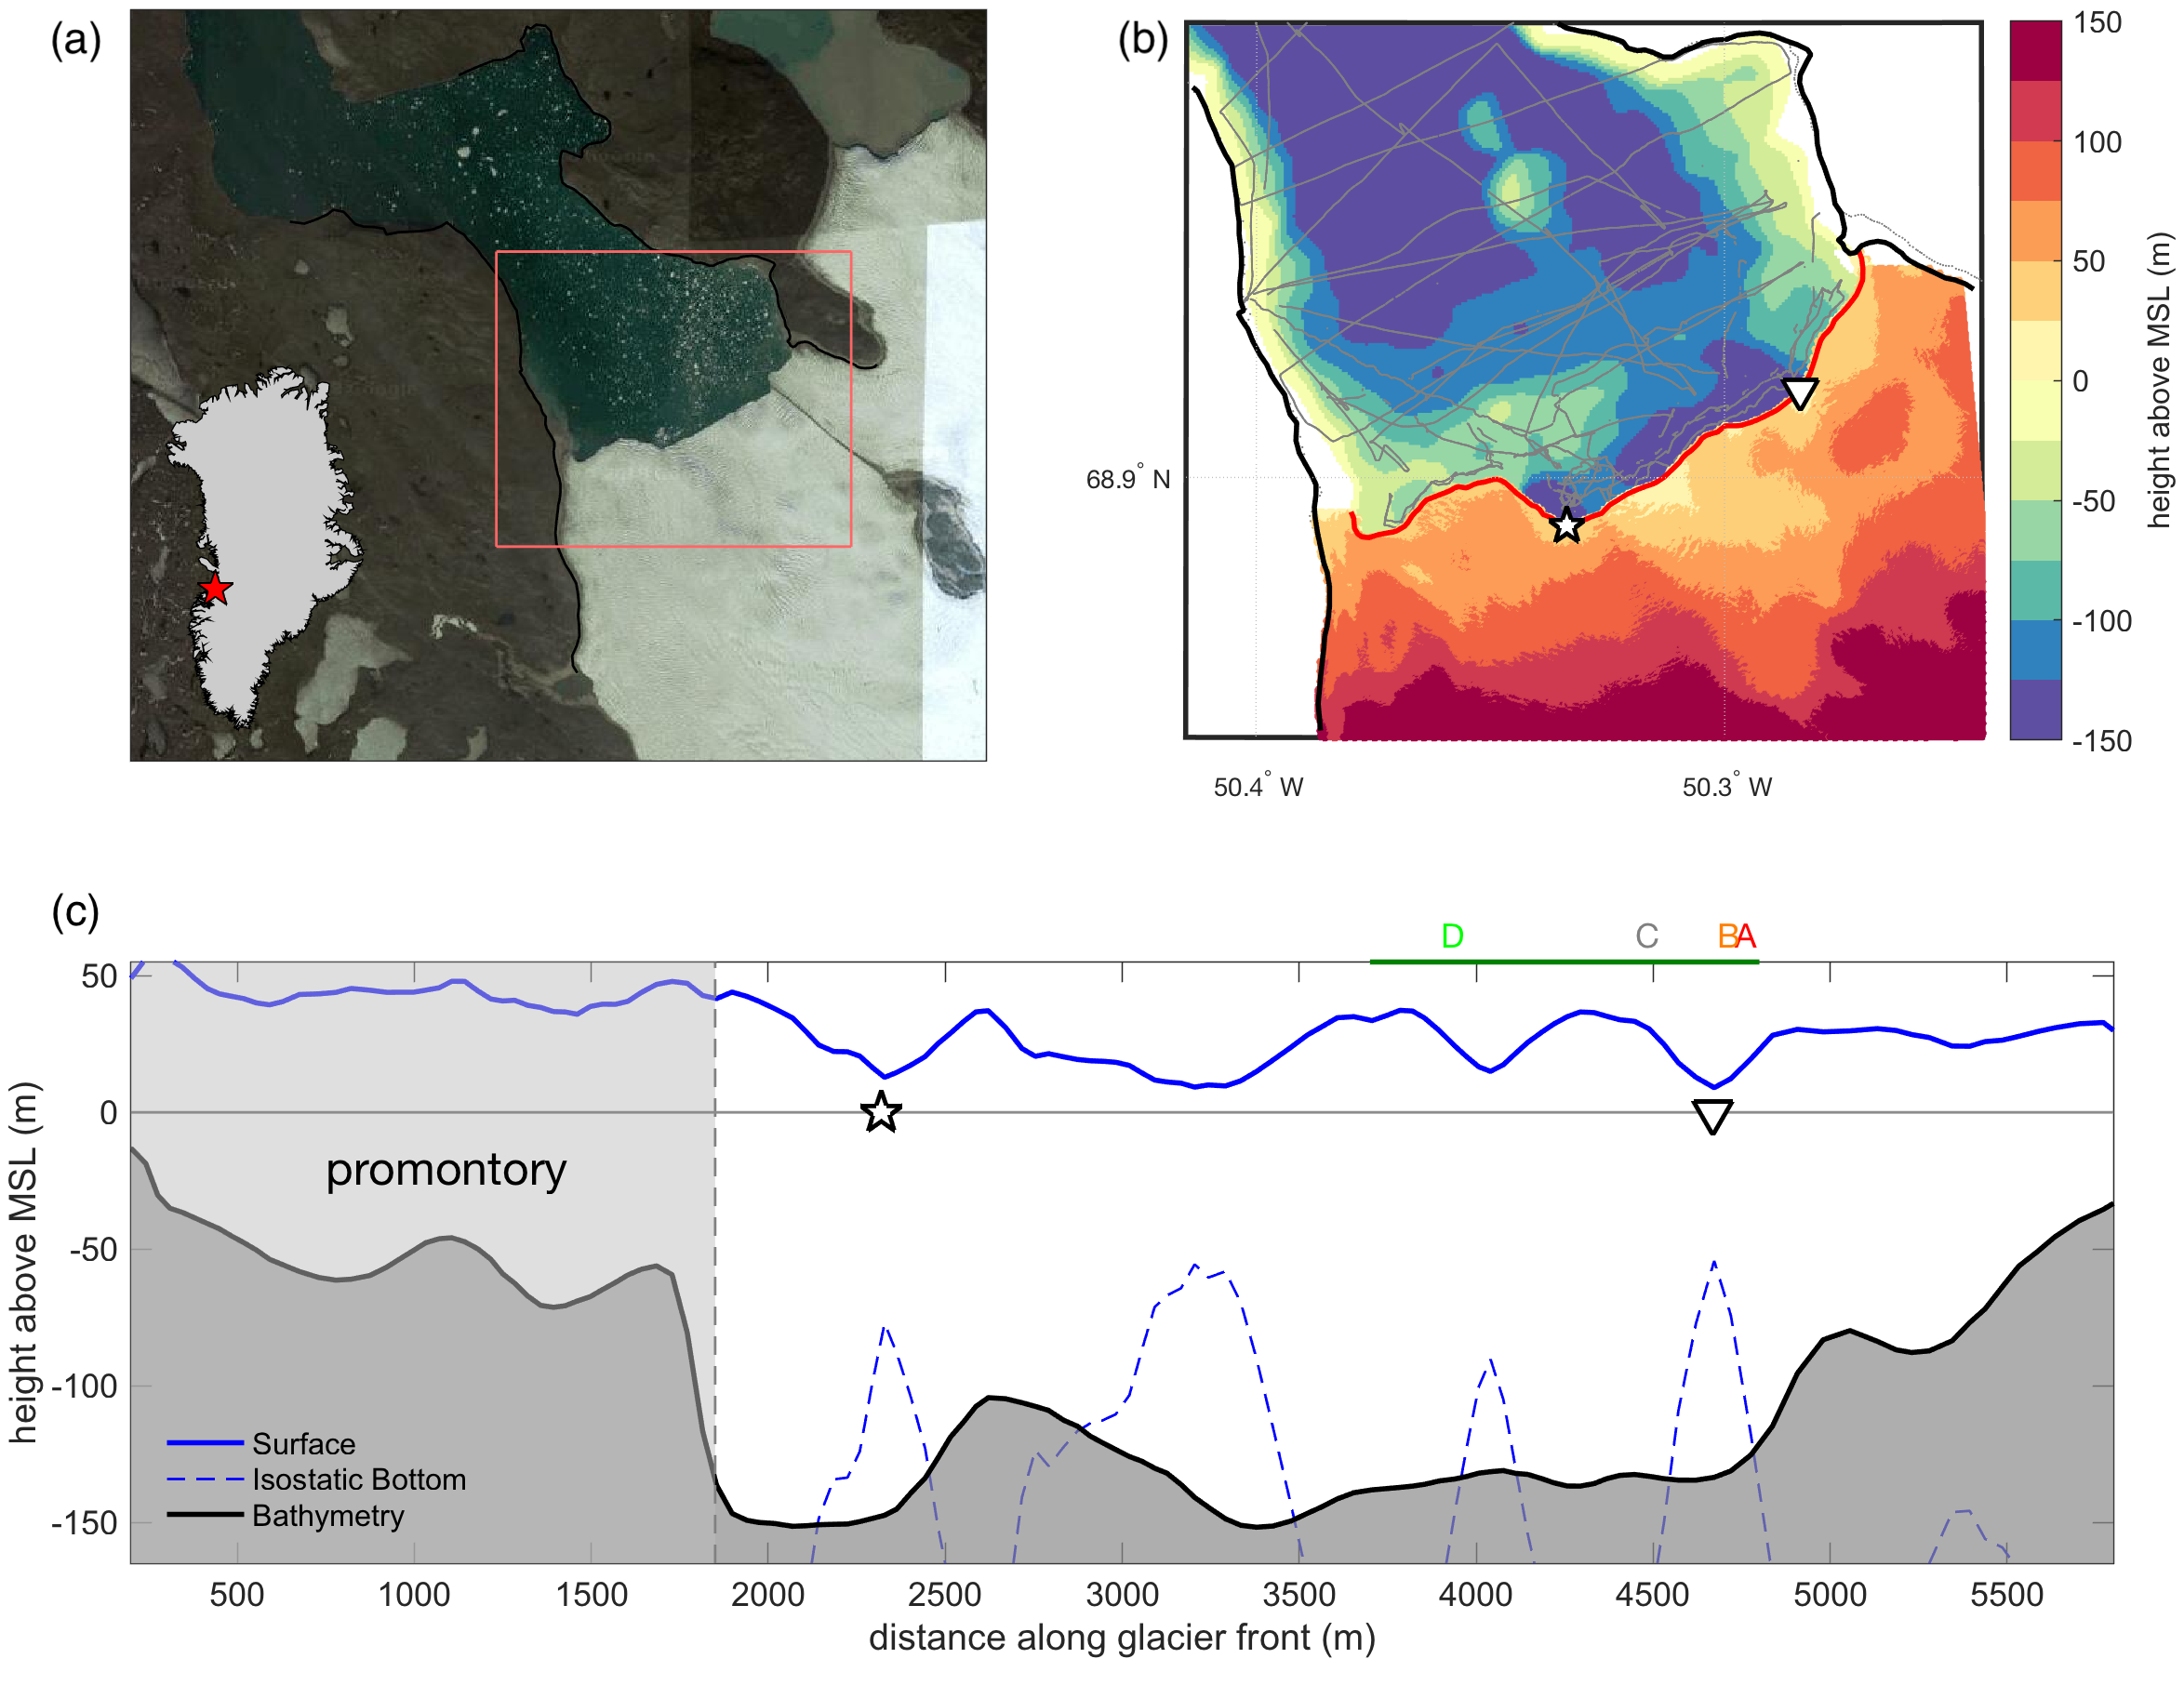
\includegraphics[width=\linewidth]{Figures/geometry4.png}
  \caption{(a) Map of the lower part of Sarqardliup Sermia, and Sarqardleq fjord. The inset of Greenland indicates the location of the glacier. (b) Gridded bathymetry from in-situ observations (readings indicated by gray dots). Also shown are the surface height from ArcticDEM, collected during an overflight on 22 March 2013; Digital Elevation Map created by the Polar Geospatial Center from DigitalGlobe, Inc. imagery. (c) Surface height (blue) and bathymetry (black) along glacier front. Also shown is the isostatic height of flotation, computed from the surface height and assuming a density 880 kg/m$^3$. Locations of two main plumes are highlighted in panels (b) and (c) by black symbols. The green horizontal line above panel (c) and the letters A-D indicate the locations of the front profiles shown in Fig \ref{fig:fronts}.}
  \label{fig:geometry}
  \end{center}
\end{figure*}

\subsection{Bathymetry} \label{bathy}

The existing bathymetry map of the fjord compiled from data collected during field work in 2012 and earlier \citep{Stevens:2016tx}, is supplemented with several additional near-terminus datasets from the 2013 field campaign. These consist of circa 39,000 depth readings taken with Jetyak and ship-mounted ADCPs. In addition, there are approximately 6000 readings from the boat-mounted NMEA bottom-range profiler and 6 readings from XCTDs deployed in the otherwise undersampled region of the main plume. Most of these readings are between 10--100 m from the glacier front. The revised bathymetry map (Fig \ref{fig:geometry}b) highlights a sill at depth $\sim$ 50 m that runs roughly parallel to the main glacier front at a distance of $\sim$1.5 km from the 2013 front position. This sill corresponds approximately to the location of the furthest advance of the glacier front in 1992. The sill furthermore separates the main basin of the fjord from a small, somewhat isolated, basin near the glacier front with slightly different water properties at depth (not shown). 

Fig \ref{fig:geometry}c shows the bathymetry at the glacier front in terms of $x$, the distance along the glacier front. The bathymetry can be split into two main regimes: For $x < 1800$ m (the promontory) the glacier is grounded in shallow waters and its surface heights are elevated substantially above floatation (see next section). From here on, we refer to the eastern part of the glacier ($x > 1800$ m) as the `main' glacier. In 2013, the front of the promontory was still coinciding with the above-mentioned sill, thus perched on bathymetry of  50 m depth or less. This part of the glacier front has also retreated since 2013 by several hundred meters (Fig S2). The main part of the glacier front is in waters of depth 130-150 m. A pronounced dip in bathymetry is found near the location of the main plume (distance $x = 2000 - 2400$ m along the front). A number of smaller dips are observed between $x = 3400 - 4700$ m. Beyond 4700 m the water depth decreases as one approaches the northeastern shoreline.

\subsection{Glacier surface topography} \label{surface}

An ArcticDEM overflight dated 22 March 2013 covers the full span of the Sarqardliup glacier front and some of the upstream region. This data provides digital elevation maps (DEMs), created by the Polar Geospatial Center from DigitalGlobe, Inc.~imagery. The data set has a horizontal resolution of 2 m and is capable of resolving individual crevasses on the glacier surface. As is also known from the field campaigns, the front of the glacier is heavily crevassed and furthermore features several pronounced dips in the surface elevation at the terminus. The ice cliff is highest (up to 50 m) and most uniform in the region of the promontory, while the main part of the glacier is much more variable with 4 distinct depressions that reach below 10 m surface elevation. A source of uncertainty is due the date of the ArcticDEM, which was collected 4 months prior to the main study period in July 2013. However, the above-water surface elevation is a relatively small contributor to the overall mass balance.

The coinciding high-resolution surface elevation and bathymetry data near the terminus enables us to compute the total ice thickness along the glacier front, $H(x)$, which allows for an estimation of the total ice flux (discussed below). 

Interestingly, the depressions in the surface elevation at the glacier front are all low enough to raise the isostatic bottom of the ice above the estimated depth of the local bathymetry. That is to say, if the glacier front was locally isostatic everywhere, the ice would be floating at the positions of the four dips shown in Fig \ref{fig:geometry}c. This assumes an average ice density of 883 kg m$^{-3}$ (obtained as a mean of the lowest and highest commonly used glacier and ice shelf densities, 850 and 917 kg m$^{-3}$). The ice would be grounded everywhere else. In particular, it is elevated substantially beyond its isostatic height in the region of the promontory. The locally-isostatic bottom of the ice is indicated in Fig \ref{fig:geometry}c (blue dashed line). It should be noted that the surrounding ice and the associated stiffness of the glacier will likely prevent the ice from assuming local isostasy everywhere along the glacier front. However, the isostatic bottom can be used to compute a lower bound on the ice thickness in regions where the ice may be floating. It may be speculated that the ice is floating in these regions due to undercutting by submarine melt (which in turn is associated with rising discharge plumes, as discussed in Section \ref{melting}). 

\section{Ice flux and retreat}

\subsection{Ice velocity and advective ice flux} \label{vels}

Several ice-velocity data fields of the lower part of the glacier are available for the years 2009 -- 2015 from InSAR data \citep{Joughin:uFAgCs4K}. The mean flow velocity at the glacier front (averaged over all available fields) is $\sim 350$ m yr$^{-1}$ with minima at the edges of the glacier. There is a notable peak in ice velocity (up to 700 m yr$^{-1}$) near the location of the main plume (Fig \ref{fig:vels}). A second stream of elevated velocities is found near $x = 4000$ m and is more pronounced somewhat further upstream. The drainage location of this second stream coincides with that of the second discharge plume. It is worth noting that the spatial distribution of velocities was remarkably consistent during summer months from 2012--2014 (Fig  \ref{fig:vels}b), followed by a substantial slow-down in 2015 (not shown). In what follows, we will consider the 2012--2014 summer (May--September) mean velocity profile along the glacier front. Using the mean July velocities instead does not change the results notably. 

%It is worth noting that the retreat of the main part of the glacier is more pronounced than that of the promontory. Aside from these differences, the rate of retreat is spatially close to uniform along the glacier front ($80 \pm 4$ m yr$^{-1}$ between 2004 and 2016). Comparing this uniformity to the highly variable calving frequencies of Fig 1 suggests a correspondingly high variability in ice velocities along the glacier front (see below).

  \begin{figure*}[t]
 \begin{center}
  \includegraphics[width=.8\linewidth]{Figures/ice_velocity3.png}
  \caption{(a) InSAR Ice velocity data near the glacier front. Shown are mean summer (June--September) values averaged over 28 velocity fields, collected during 2012--2015. Note that there is a consistent data gap near the promontory. The shading represents the velocity magnitude, the arrows the flow direction. (b) Velocity profiles along the glacier front. Here, as in all figures, the perspective is with the direction of ice flux into the page.}
  \label{fig:vels}
  \end{center}
\end{figure*}

The magnitude of the summer ice velocity $v_i$, shown in Fig \ref{fig:vels}b, together with the ice thickness profile $H(x)$, allows for an estimate of total advective ice flux (Fig \ref{fig:flux}). This assumes plug flow, i.e., that the ice velocity is approximately constant from the surface to the ice--bedrock interface, which is thought to be a good approximation for fast-flowing tidewater glaciers \citep{Meier:te}.
The uncertainty in ice thickness associated with the glacier potentially floating at several points along the front is illustrated by the shaded areas in Fig \ref{fig:flux}. In the figure the upper bound of the ice thickness assumes a fully grounded glacier front, while the lower (dashed) bound assumes local isostasy everywhere.
Naturally, the ice flux is highest when assuming a fully grounded glacier, while a partially floating glacier front would have a correspondingly reduced flux. 

%The mean summer ice flux along the glacier front is shown in Fig \ref{fig:flux}.

  \begin{figure*}[ht!]
 \begin{center}
  \includegraphics[width=.8\linewidth]{Figures/ice_fluxes2}
  \caption{(a) Mean July ice velocity along the glacier front in red (left vertical axis). In blue (right vertical axis) is shown the estimated ice thickness along the glacier front, obtained by computing the difference of the surface and bathymetry profiles of Fig 1(c). The dotted red line shows the ice thickness at the glacier front assuming the ice is locally in isostatic equilibrium everywhere. (b) Ice flux along the glacier front (in black), computed from the product of velocity and thickness (shown in panel a). The shaded gray areas are the ice-flux range due to potential flotation. This corresponds to the thickness ranges indicated as red shaded areas in panel a. Also indicated are the approximate locations of the two known plumes (star and circle), which coincide with two areas of flotation. 
% It may be speculated that there are further secondary or more transient plumes near the regions $\sim 3300$ m and $\sim 4000$ m along the glacier front.
}
  \label{fig:flux}
  \end{center}
\end{figure*}


  \begin{figure*}[ht!]
 \begin{center}
  \includegraphics[width=\linewidth]{Figures/retreat2.png}
  \caption{Seasonal advance and retreat of glacier front. (a) 15 front profiles acquired from Feb to Sep 2013, color-coded as in the legend. The thick red and blue profiles represent the May--June and Sept averages, respectively. (b) Mean front position, shown as an anomaly from the yearly mean position. 2012 values are shown in gray, 2013 in black. The spring profiles used in panel (a) are highlighted in red, fall profiles in blue. The vertical dashed lines demarcate the period from July 12-31 during which calving was observed. (c) Retreat rates along the glacier front. The dashed line represents the spring -- fall mean retreat rates; the solid line that of July 9 -- 31.}
  \label{fig:retreat}
  \end{center}
\end{figure*}

\subsection{Changes in glacier front position} \label{fronts}

%\subsubsection{Seasonal advance--retreat cycle}
Superimposed on the above-mentioned longterm retreat of the glacier front over the past decades (Fig S2) we observe a seasonal advance--retreat cycle during 2012 and 2013. A total of 27 front positions from Jan--Oct 2012 and 2013 were digitized from TerraSAR-X satellite images. The 15 profiles from 2013 are shown in Fig \ref{fig:retreat}a. Both years exhibit a clear, albeit modest, seasonal cycle in terminus migration, with a spatial-mean advance of roughly 30 m from January through April/May, followed by a more rapid retreat from June to September of circa 80 m (Fig \ref{fig:retreat}b). However, there is substantial along--glacier variability in this cycle. Near the edges of the glacier, and in particular at the promontory, the glacier exhibits a much reduced advance--retreat cycle, and more variable regions are found in the main dynamic section of the glacier. 

We define $R(x)$ as the rate of retreat of the glacier front at location $x$, in m yr$^{-1}$. $R(x)$ is computed as the rate of retreat perpendicular to the initial glacier front. The most rapid retreat in 2013 was observed at the time of the July study period. Fig \ref{fig:retreat}b shows the spatial-mean seasonal retreat rates $\langle R \rangle$ for 2012 and 2013, with profiles from 9 and 13 July 2013 highlighted in green. Such rapid retreat is spatially highly variable (Fig \ref{fig:retreat}c) and strongly impacted by sporadic but large individual calving events. Longer-term mean retreat rates, computed from average spring and fall glacier front positions may therefore be more representative (Fig \ref{fig:retreat}c) . We note that the spring versus fall retreats of 2012 and 2013 were spatially anti-correlated, in other words, regions that saw a large retreat in 2012 experienced little or no retreat in 2013, and vice versa (Fig S3). 

\section{Ablation and mass balance along the glacier front}

In order for the mass budget along the glacier front to be balanced, the sum of advective ice flux and frontal retreat must be balanced by total ablation (i.e., by the sum of melting and calving fluxes). Here we consider a steady state, vertically averaged balance. At a given point along the glacier front this can be written as
\be
H\left(R + v_i \right) = D\bar{M} + C. \label{eq:mb}
\ee

%We consider a glacier front with along-front coordinate $x$ and ice thickness $H(x)$. In this study, ice thickness is estimated from in situ bathymetry readings taken close to the terminus (see Section \ref{bathy}) and satellite-derived surface elevations (see Section \ref{surface}).  We assume that glacier front position does not change over the study period to an extent that would substantially change $H(x)$ -- ice thickness is therefore considered constant in time. 


%This is estimated from satellite-derived frontal positions (see Section \ref{fronts}).  
% The first term on the right represents the volume flux from ice advection. Here, $\vec{v}_i(x)$ is the ice velocity across the glacier front at $x$, computed from InSAR imagery (see Section \ref{vels}). 
 The first term on the right represents the ice loss due to underwater melting, where $D(x)$ is the draft of the glacier and $\bar{M}(x)$ is the depth-averaged melt rate. $\bar{M}$ is derived from in-situ hydrographic observations, in concert with a high-resolution numerical model (see Section \ref{melting}). The final term on the right hand side of equation \eqref{eq:mb} is the volume loss due to calving. This is estimated from in-situ pressure sensors (see Section \ref{calving}), and presents the least well constrained term of equation \eqref{eq:mb}.

In what follows we consider the volume flux across the glacier front during the summer of 2013. We make the assumption that this flux was steady during the study period and ignore time-dependencies of the individual terms in equation \eqref{eq:mb}.

%If we take the movement of the glacier front, $R$, to be negative (i.e., retreating) everywhere, we can write $R  \equiv -|R|$. This is true for the mean spring--fall retreat and a good approximation for the July retreat, as shown in Fig \ref{fig:retreat}c. We can then rewrite equation \eqref{eq:mb} as 
%In words, the sum of ice advection and summer retreat is equal to the total ice ablation, which given by the sum of melting and calving fluxes.
%The individual terms of equation \eqref{eq:mb2} are summarized in Fig \ref{fig:ablation}. 
\subsection{Calving frequency and distribution} \label{calving}

Calving events were detected over a 19-day period from July 12 to July 31 2013, using two pressure sensor moorings located on the western and eastern banks of the fjord, each at a distance roughly 2 km from the nearest point along the glacier front (Fig \ref{fig:calving}a). The dispersion of waves that are created by individual calving events can be inverted to estimate the distance between the mooring and the origin of the wave. Wave packets that are detected by both moorings can be used to triangulate the time and position of the corresponding calving event \citep{MINOWA:2018et}. The method was previously validated against a photography-derived calving record by Richards et al.~(2018), and good correspondence was observed. The study by Richards et al.~(2018) furthermore provides a detailed description of the method, as well as of the collection and analysis of the current dataset.

In total, 336 calving events were identified using this method over the period that both sensors were recording. Fig \ref{fig:calving}b shows the location and an estimated magnitude of the individual events. The calving frequency distribution along the glacier front is illustrated in Fig \ref{fig:calving}c.

 A pronounced peak in frequency is found at the promontory, where particularly shallow bathymetry causes the glacier to be elevated substantially beyond its isostatic height of flotation. With its high ice cliffs the promontory can be regarded as a region that is subject to a rather different calving regime, compared to the rest of the glacier. 
% In what follows we will focus on the more dynamically active main part of the glacier front to the northeast of the promontory. 
 
 For the main part of the glacier, we observe a peak in calving activity at a distance  $x \approx 2400$ m along the glacier front, which corresponds to near the concave bend in the glacier front (Fig \ref{fig:calving}b). A second peak in calving activity is found around $x \approx 4300 $m. The calving activity is lowest at the northeast edge of the glacier.
 
 Even though this dataset presents a rather accurate record of calving frequencies, it remains challenging to infer a total volume of calved ice. This is due to the different modes of calving (e.g., ice cliff calving versus submarine calving), as well as the different shapes of calved ice blocks and the differing heights from which they fall (or depths from which they rise). Distinguishing between these events from the pressure sensor data is a difficult task and beyond the scope of this study. The pressure sensors do record an amplitude of the incoming wave packet associated with a given calving event, and assuming that this amplitude is correlated with the size of the calved ice we can estimate a relative calving volume (black curve in Fig \ref{fig:calving}b). However, since a small cone-like shaped ice block can act as a more efficient wave generator than a large flat piece of ice \cite[N. Pizzo, personal communication,][]{BUHLER:2007db}, it is difficult to ascertain a direct relation between wave amplitudes and calving volume. In what follows we therefore only consider the calving frequency record and will scale this record such that the resulting mean calving flux approximately closes the mass budget at the glacier front.
 
   \begin{figure*}[h]
 \begin{center}
  \includegraphics[width=\linewidth]{Figures/calving_figure2.png}
  \caption{(a) Close-up of glacier front and adjacent fjord, with the red rectangle outlining the region of interest (next panel) and red stars indicating the location of the wave moorings (see text); (b) spatial calving distribution as estimated from pressure sensor data; the shaded rectangle indicates the promontory at the western part of the glacier front (see text);  (c) calving count along glacier front, obtained as total number of calving events detected within a 300 m running window along the glacier front (with bins centered on the bars); the promontory is again indicated by the shaded gray area. Also shown is an estimate for the relative calving volume, computed from the product of the frequency of calving events at a location $x$, and the corresponding magnitudes of the detected waves (right axes, black line).}
  \label{fig:calving}
  \end{center}
\end{figure*}


\subsection{Submarine melting} \label{melting}

The submarine melting regime at Sarqardleq Sermia has been studied in detail by Slater et al. 2018 and is briefly described here. Submarine melt rates are thought to respond primarily to fjord water velocity and temperature adjacent to the calving front. Given the great difficulties of directly measuring submarine melt rates, it is instead usual to estimate fjord water velocity and temperature  and then employ a parameterization to estimate melt rates. Slater et al. 2018 used both data collected close to the calving front and numerical modeling to estimate water properties and this submarine melt rates at Sarqardleq Sermia, (see their Fig. X). There is good agreement between the melt rates estimated with the numerical model and with the observations. Here, we only consider the modeled melt rates, which have the advantage of covering the whole extent of the glacier front (unlike rates inferred from observations, which have data gaps in and around the plumes). 

The relevant term for the frontal mass budget is the depth-averaged melt rate (Fig \ref{fig:ablation}b). However, we also consider the possibility for melting to have a dynamic impact on calving, in which case the vertical profile of the melt rates becomes of interest. The 2D melt pattern along the glacier front and corresponding maximum melt rates are shown in Fig. S4). 

There is huge spatial variability in submarine melt rates along the calving front. Submarine melt rates are highest (both in a depth-averaged and maximum sense) within the two plumes where the discharge of buoyant surface meltwater from beneath the glacier gives high water velocities. Outside of the two plumes melt rates are much smaller in a depth-averaged sense, however the lateral circulation excited by the plumes combines with warm surface waters to give high melt rates near the surface outside of the plumes as can be seen in Fig S2 (Slater et al. 2018).

\subsection{Frontal mass budget}

To compare the different terms in the overall mass budget, we consider the retreat rate as computed from the two fronts measured on 9 and 31 July 2013, since this is almost the exact time window of the calving observations (12 -- 31 July).  For the advection term we use the July average over the years 2012 -- 2014, since the July 2013 ice velocity fields have some notable data gaps at the glacier front. However, as discussed above, there is little interannual variability in $v_i$ over these years, so the 3-yr mean likely gives a close approximation to the July 2013 velocity field. Front retreat, advective flux, and their sum (i.e., the left hand side of equation \ref{eq:mb}) are shown in Fig \ref{fig:ablation}a. Melt fluxes, estimated calving volumes, and their sum (i.e., the right hand side of equation \ref{eq:mb}) are shown in Fig \ref{fig:ablation}b. 

Integrated along the glacier front we estimate the following frontal mass budget terms (for the main part of the glacier); (i) Advection: 0.2 Gt yr$^{-1}$, (ii) Retreat: 0.3 Gt yr$^{-1}$, (iii) Melting: 0.03 Gt yr$^{-1}$, (iv) Calving: 0.5  Gt yr$^{-1}$. In summary, the glacier loses mass almost exclusively due to calving, apart from in very localized areas near the subglacial discharge plumes. However, the localized melting likely still plays a central role in the glacier's mass balance since it can drive rapid calving, as discussed below. 
 
%mean advective flux is 78568 
%max advective flux is 106151 
%
%max retreat flux is 213919 
%mean retreat flux is 101697 
% 
%plume melt flux is 154138 
%off-plume melt flux is 4560  
%mean melt flux is 10373 
% 
%max calving flux is 244872 
%mean calving flux is 164766 
% 
%mean ablation flux is 175138 
%mean loss flux is 181089 
%
%total retreat rate is 3.155655e+08 
%total advective rate is 2.437963e+08 
%total calving rate is 5.112684e+08 
%total melt rate is 3.218739e+07 


   \begin{figure*}[ht!]
 \begin{center}
  \includegraphics[width=.75\linewidth]{Figures/ablation_vs_loss3.png}
  \caption{Volume balance along the glacier front. (a) The green line represents the July 2013 retreat rate and the blue line the advective ice flux. The sum of these two terms (black) must be equal to total ablation. (b) Melt flux (light red) and calving flux (dark red). The total ablation, i.e., the sum of melting and calving, is shown by the gray line. Note that the calving flux has been scaled to approximately close the budget. (c) Approximate closure of the volume flux budget along the glacier front. The black line shows the sum of ice advection and retreat as in panel (a), while the gray line shows the total ablation as in panel (b).
}
   \label{fig:ablation}
  \end{center}
\end{figure*}

%For the melting flux we use the modeled depth-averaged values for summer 2013, as discussed in Section \ref{melting}. 

%Fig 6b relates the total ice flux to the calving frequencies along the glacier front. We find that there is overall a good correspondence between the ice flux and the calving rates in the main part of the glacier front. For this part, the highest calving rates are observed near the location of the main plume, which coincides with the region of highest ice flux (green star). Interestingly, the secondary peak in calving rates (around $x = 4000$), which also corresponds to the secondary peak in ice velocities, does not stand out as a region of high ice flux. Furthermore, this region does also not coincide with the location of the secondary plume (green circle), although it does coincide with a dip in the surface elevation and with the secondary peak in ice velocity. This suggests that the ice velocity in itself might be more closely linked to calving rates, rather than the ice flux. It is also not clear whether the calving rates are better correlated with the grounded or with the floating ice profile.  

\section{Discussion -- spatial variability and the impact of melting on overall ablation}

\subsection{High spatial variability along the glacier front}

A striking feature of almost all components of this multipartite dataset is their high spatial variability along the glacier front. 

The ice thickness at the front ranges from thin ($<40$ m) sections near the northeast edge to $\sim 100$ m along the promontory and  up to 192 m near the main plume, with substantial variations throughout. Overall, we observe a mean thickness of 128 m with a variability  of $\pm 38$ m (1 standard deviation). 

We find that the advective flux is suppressed at the promontory and highest near the outflow location of the main plume, with a second smaller peak near the secondary plume (Fig \ref{fig:flux}). 

The retreat rates are overall of comparable magnitude to the advective flux. However, these rates are extremely variable, in particular the observed July 2013 rates, which exhibit three regions of enhanced retreat, two of which are close to the two discharge plumes, with peaks at $x = 2400$ and $4400$ m (Fig \ref{fig:retreat}c). 

Calving frequencies, on the other hand, are strongly enhanced at the promontory, which -- given the reduced advection and retreat in this area -- suggests that calved pieces are in general smaller at the promontory. Even though calving rates are overall lower for the main part of the glacier, we observe two local maxima, slightly offset from the plumes (Fig \ref{fig:ablation}b). The lowest calving rates are found between the two plumes and in the region farthest from both plumes. 

The two peaks in depth-averaged melt flux (Fig \ref{fig:ablation}b), co-located with the two discharge plumes at $x = 2300$ and $4500$ m, are just offset from the two peaks in frontal retreat and calving. The \textit{maximum} melt flux value ($1.5 \times 10^5$ m$^2$ yr$^{-1}$) is slightly higher than the \textit{mean} retreat and advective flux values ($1.0 \times 10^5$ and $0.8 \times 10^5$ m$^2$ yr$^{-1}$). Outside the two plumes the mean melting flux ($0.04 \times 10^5$ m$^2$ yr$^{-1}$) is an order of magnitude lower than inside the plume and than the other terms. 

In order to approximately balance the total ablation with the sum of ice advection and retreat, we scale the relative calving rates by a constant factor. This gives a mean calving flux of $1.7 \times 10^5$ m$^2$ yr$^{-1}$, which is an order of magnitude larger than the estimated mean melting flux of $0.1 \times 10^5$ m$^2$ yr$^{-1}$. 

[XX Donald: quick discussion of how to scale melt params to close budget without calving?]

\subsection{Impact of melting on overall ablation}

Although the volume of ice lost through submarine melting is small, melting may still play an important role in the glacier's frontal mass balance: since it is highly focused on discrete regions of the glacier front melting can lead to sharp incisions in the front profile that may be significant drivers of calving.

Slater et al (2018) recently found that fjord recirculation driven by subglacial discharge plumes can cause substantial near-surface melting along the glacier front (away from the discharge locations of the plumes, see Fig S3). This near-surface melting has in turn been suggested as a potential driver for large calving events at glacier fronts that are floating or close to floating \cite{Wagner:2016hj}. Preferential near-surface melting at the glacier front leads to a horizontal `wave-notch' near the sea surface which in turn causes erosion of the above-water ice cliff. As a result, the front of the glacier is left with an underwater protrusion (or `ice foot'). This frontal profile is statically unstable, since the ice foot is net buoyant and exerts bending stresses on the glacier. Calving events occur when such stresses surpass the yield strength of the terminus. This process has also been observed on icebergs in temperate waters \cite{Scambos:2005un,Wagner:2014uz}. 

  \begin{figure*}[t]
 \begin{center}
  \includegraphics[width=.8\linewidth]{Figures/front_shapes}
  \caption{(a) Multibeam sonar data of glacier front from jetyak (26 July 2013). The transect shows a part of the eastern side of the glacier (distance along glacier front, $\sim 4000 - 4800$ m). Data is color-coded by depth. Indicated are the locations of the two cross-sections in panels b and c. (c) and (d) Example cross-sections far from plume, showing a retreat of the glacier front toward sea level. (a) and (b) Example cross-section near subglacial plume, exhibiting characteristic undercutting.}
  \label{fig:fronts}
  \end{center}
\end{figure*}

At Sarqardliup, the glacier front was indeed found to feature large sections with underwater protrusions. During the 2013 field season an autonomous surface vehicle (the Woods Hole Oceanographic Insitution ``Jetyak") was deployed \citep{Kimball:kr,Mankoff:2016jp}.
Among other instruments, the Jetyak carried a multibeam sonar that was mounted sideways facing the glacier, which collected three-dimensional maps of the underwater portion of the glacier front. Further details of the Jetyak's operation and data are found in \cite{Kimball:kr}. Here, we highlight several characteristic frontal profiles. Fig \ref{fig:fronts} shows a point-cloud transect of the northeastern flank of the glacier, as well as four vertical line profiles at different locations along the transect. 

The first two profiles (A and B) are placed near the secondary plume. Both profiles are marked by two features: (i) a sloped upper 20--25 m, which results in the above-water cliff of the glacier being set back by 10--20 m, relative to the most ocean-ward point of the glacier face. (ii) Below 40 m we observe up to 10 m of undercutting, such that the protrusion beyond the above-water cliff is most pronounced at depths 20-40 m, and the ice is substantially eroded at greater depths. This is likely caused by warmer fjord waters that are entrained by the rising subglacial plume \citep{Fried:2015bc,Slater:2017dm}, and that preferentially melt the deeper parts of the glacier front. Profiles C and D, which are located far from the plume, also feature said underwater ice protrusion, however, they show no signs of undercutting. 
%While the slope is confined to the upper 30 m in profile D (similar to profiles A and B), the protrusion in profile C is rather steadily growing until the maximum measurement depth of about 80 m. 

   \begin{figure*}[ht]
 \begin{centering}
  \includegraphics[width=.8\linewidth]{Figures/calving_melting_cartoon.png}
  \caption{Schematics of two distinct ablation regimes. (a) Melt-dominated regime: the vertical structure of melting due to a rising subglacial discharge plume which entrains warm ambient water results in substantial undercutting of the glacier front (as in profiles A and B in Fig \ref{fig:fronts}). These front profiles likely do not cause large calving events with calving mostly confined to the smaller subaerial cliff. Profiles are drawn for an earlier time $t_1$ and a later time $t_2$ by which the glacier has retreated mostly due to melting. (b) Calving--dominated regime: here the growth of sizable and buoyant underwater feet can accelerate calving, with the melt contribution confined to a small region near the water surface (the `wave-notch'). Again, profiles are shown at $t_1$ and $t_2$ (pre and post-calving), as part of the `footloose' calving cycle.}
  \label{fig:regimes}
  \end{centering}
\end{figure*}

The bathymetry reaches depths of around 130 m for this part of the glacier and the bottom 50 m or so are unfortunately not captured by the multibeam sonar. However, the profiles located near the melt (A and B) can be expected to be further undercut below the observed range \citep{Fried:2015bc}. It is likely that profiles C and D, on the other hand, are representing sizable ice feet which exert bending stresses that enhance the calving flux in this region. 

Finally, it is also possible that the regions adjacent to the meltwater plumes are more prone to calving since the high melt rates at the plumes cause vertical incisions in the glacier front. These in turn would reduce the transverse (i.e., along-front) stability of the terminus, and trigger further calving. A surface expression of these vertical incisions in the glacier front can be found near the main plume in the front profile of August 2012 (Fig S2).

In summary, from these observations we propose that there are two distinct regimes driving ablation at Sarqardliup: (a) melting-dominated ablation in spatially confined regions near the discharge plumes, and (b) calving-dominated ablation in the regions away from the plumes (which may be enhanced by horizontal melt incisions). This is further supported by the local minimum in calving activity at the location of the main discharge plume (Fig \ref{fig:ablation}b). The two ablation regimes are summarized in a schematic in Fig \ref{fig:regimes}.

%The region of the promontory is found to be in a notably different calving regime. Even though it features some of the lowest ice flux (a result of thin ice and low velocities) it is marked by the highest calving rates. This can be explained by that fact that here the ice rises high above its flotation hight and the resulting tall ice cliffs lead to high calving rates. This highlights one of the limitations of the calving detection method in its current form: while the promontory features high rates of calving, these calving events are likely small in their calving volume, but often efficient in generating waves, since they fall from greater heights. This is also likely a cause for the elevated calving rates at $x\geq5000$ (relative to the ice flux), where the glacier rides up onto the banks of the fjord. In future, it may be possible to refine the calving detection method such that it accounts for the type of calving by a more advanced analysis of the dispersion of the incoming wave packet. This may allow for a more detailed characterization of the different calving regimes governing different glaciers or different sections of a given glacier as in the present case.

%The calving-detection method does allow for a rough estimate of the calving event magnitude by looking at the size and amplitude of the incoming wave packet (see Richards et al, 2018). For the present dataset the magnitude is approximately linearly related to the frequency of calving. That is to say, during periods of higher or lower calving rates, the estimated calving volume is proportionally higher or lower. If we assumed that the thus estimated calving volume, as well as the computed ice flux, were perfect we would be able to calculate the melt rates (per unit glacier front) as simply the residual between calving volume and flux. However, with the given limitations of the data presented, such a calculation is not yet feasible. 

\section{Conclusion}

We have presented a multi-faceted dataset of a Greenland tidewater glacier and its surroundings. The unique dataset enables us to investigate the individual terms that determine the mass balance along the glacier front. 

We find that the individual terms that comprise the glacier's frontal mass budget are marked by high spatial variability. Ice velocities feature maxima that coincide with troughs in the bathymetry and locations of subglacial discharge plumes. The retreat rates are spatially particularly variable when calculated over shorter periods of time (days to weeks). Spikes and troughs in glacier retreat rates over such short timescales are likely dominated by somewhat stochastic calving events. Melting, on the other hand, is more consistent in time and can be expected to only feature gradual changes. 

%We find that in terms of overall volume loss of ice, melting is dominated by calving at Sarqardliup, except in the vicinity of the plumes. 
%However, we hypothesize that calving is substantially enhanced by the localized and highly focussed melt pattern. 
The spatial structure of the observed processes suggests the presence of two distinct ablation regimes: a melting-dominated one near the discharge plumes and a calving-dominated regime away from the plumes. Although the total melt volume is small compared to the other terms in this mass balance, melting does likely play an important role by indirectly driving calving in the off-plume regions of the glacier front.

% This work highlights the substantial degree of spatial variability in the retreat, advection and ablation processes that determine the migration of the glacier front, even on the small ($\sim$100 m) scales of a medium-sized Greenland tidewater glacier. 
 
 If calving is indeed dependent on melt rates, this may have far-reaching implications for the overall stability of the glacier. It is commonly assumed that a glacier's calving behavior is by-and-large determined by its geometric constraints (e.g., bathymetry) and the integrity of the ice near the terminus (e.g., presence of surface melt ponds or degree of crevassing). Melt-driven calving, on the other hand, will be impacted by changes in water temperatures and fjord circulation patterns. This would imply that the overall stability of tidewater glaciers may be more dependent on the local ocean conditions than sometimes assumed.

\section{Acknowledgements}
Geospatial support for this work provided by the Polar Geospatial Center under NSF OPP awards 1043681 and 1559691. DEMs provided by the Polar Geospatial Center under NSF OPP awards 1043681, 1559691 and 1542736.

\vspace{.2in}
%\bibliographystyle{agufull08} 
\bibliographystyle{unsrtnat} 
%\bibliographystyle{naturemag} 
\bibliography{calving}  

\clearpage

\section*{Supplementary Figures}

\setcounter{figure}{0}    
  \begin{figure*}[h!]
 \begin{centering}
  \includegraphics[width=\linewidth]{Figures/bathy_data.png}
  \caption{Locations of bathymetry readings used to create map in Fig 3a. Blue dots are new data added for this study, while black dots were first presented in \cite{Stevens:2016tx} and are also used for BedMachine3 \cite{Morlighem:2017fd}. The red line is the glacier front in August 2013.}
  \label{fig:bathy_data}
  \end{centering}
\end{figure*}

  \begin{figure*}[h]
 \begin{center}
  \includegraphics[width=.85\linewidth]{Figures/longterm_retreat.png}
  \caption{Longterm retreat of the Sarqardliup glacier front. While only profiles from 12 years between 2004 and 2016 are shown in panel (a) for clarity, panel (b) gives the evolution of the mean front position since 1975.}
  \label{fig:longterm_retreat}
  \end{center}
\end{figure*}

  \begin{figure*}[h]
 \begin{center}
  \includegraphics[width=.85\linewidth]{Figures/retreat_2012_2013.png}
  \caption{Spring--fall retreat rates for 2012 (blue), 2013 (red), and the average over both years (black). Note the anti-correlation between the 2012 and 2013 retreat rates.}
  \label{fig:retreat1213}
  \end{center}
\end{figure*}


  \begin{figure*}[h]
 \begin{center}
  \includegraphics[width=\linewidth]{Figures/outplumemelt.png}
  \caption{XX Donald: alter this to just show the modelled results? }
  \label{fig:plumemelt}
  \end{center}
\end{figure*}

%
%  \begin{figure*}[h!]
% \begin{centering}
%  \includegraphics[width=\linewidth]{Figures/FigS2}
%  \caption{July surface ice velocity maps. The different rows correspond to different years (2012 - 2015). Panel (i) shows the velocities along the southwest--northeast transect as indicated in panels (a-h). Clearly visible are the velocity peak in the region of the main plume (longitude 50.32$^\circ$W) and a secondary region of elevated velocity near the discharge location of the second plume (longitude 50.28$^\circ$W). The interannual variability in ice flow velocities is small (relative to the along-front variability).}
%  \label{fig:S2}
%  \end{centering}
%\end{figure*}
%
%\subsection{Hydrographic properties}
%
%Three transects of CTD casts were collected at distances of 100 -- 150 m from the glacier front on 25, 26, and 31 July 2013 (see Fig S3). Each transect consisted of 7 -- 10 casts. A consistent general structure of both temperature and salinity profiles is observed, with the warmest waters confined to the top 20 -- 30 m, followed by a slightly cooler layer between 30 -- 70 m and then warmer waters again beneath 70 m depth. The warm surface waters are in agreement with the higher melt rates in this region inferred from the multibeam ice profiles (Fig 3). Salinity is continuously increasing with depth, ranging from a fresh 26 psu near the surface to 34 psu at depth. There is substantial variability in the temperature and salinity profiles between the different days. For example, the 26 kg/m$^3$ isopycnal is depressed by approximately 20 m between July 25 and 26 (from 40 to 60 m) and a further 20 m between July 26 and 31. This is accompanied by a corresponding cooling and expansion of the cold middle layer. Furthermore, the outcropping of the isopycnal at $x = 1800$, indicative of the surfacing of the main plume, is only observed in the latter two transects, but not in the first. Finally, there is no clear evidence of the secondary plume in these profiles, unlike in the CTD casts taken in 2012 \citep[][their Fig 4]{Stevens:2016tx}.
%
%
%\subsection{Diurnal cycle, surface air temperatures, tides, and subglacial discharge}
%
%A notable advantage of the pressure-wave detection method is that it allows for a continuous record of calving events (unlike aerial or terrestrial photography which are restricted to daylight hours). It may be expected that calving events are more likely to occur in the afternoons when temperatures have been above freezing for a number of hours. However, no such (or any other) discernible diurnal signal is found in the calving record (see Fig S4). Similarly, we investigated whether the occurrence of calvings during the 3-week study period may have been influenced by other environmental factors. Fig S5 thus shows the (normalized) calving frequency timeseries and compares it to the 2-m surface air temperature data from the two nearest meteorogical stations (Illulisat and Qasigiannguit). However, no significant correlation is apparent, which suggests that the observational window was too short to establish any significant relations. This would imply that calving frequencies at Greenland's tidewater glaciers (or at least in this region), respond to changes in air temperature only on timescales that are significantly longer than a week, if at all. Analogous results where found when comparing calving frequencies to the slope and amplitude of local tides (not shown) and estimated subglacial runoff (shown in Fig S6, using RACMO output for this catchment basin from \cite{Stevens:2016tx}).
%
%
%  \begin{figure*}[h!]
% \begin{centering}
%  \includegraphics[width=\linewidth]{Figures/FigS3}
%  \caption{hydrography data}
%  \label{fig:S3}
%  \end{centering}
%\end{figure*}
%
%  \begin{figure*}[h!]
% \begin{centering}
%  \includegraphics[width=.7\linewidth]{Figures/FigS4}
%  \caption{Calving events binned according to hour of day: (a) in bins of 6 hour length and (b) hourly bins. No discernible diurnal cycle here.}
%  \label{fig:S3}
%  \end{centering}
%\end{figure*}
%
%  \begin{figure*}[h!]
% \begin{centering}
%  \includegraphics[width=.7\linewidth]{Figures/FigS5}
%  \caption{Normalized DMI 2-m surface air temperature data (daily means) for July 12 - 31. The blue and green circles correspond to data from the two nearest meteorological stations at Ilulisat and Qasigiannguit, respectively. Also shown are the (normalized) daily calving frequencies (red squares). No significant correlation between the temperature data and the calving frequencies is found here (as indicated by the r and p-values in the legend).}
%  \label{fig:S3}
%  \end{centering}
%\end{figure*}
%
%  \begin{figure*}[h!]
% \begin{centering}
%  \includegraphics[width=.9\linewidth]{Figures/FigS6}
%  \caption{Comparison with estimated subglacial discharge from RACMO output (see main text).}
%  \label{fig:S3}
%  \end{centering}
%\end{figure*}

%\subsection*{\sf Acknowledgements}
%I'd like to thank my parents for giving me two middle names.

\end{document}
